% -----------------------------------------------------------------
% Vorlage fuer Ausarbeitungen von
% Bachelor- und Masterarbeiten am ISS
% 
% Template for written reports or master theses at the ISS
% 
% For use with compilers pdflatex or latex->dvi2ps->ps2pdf.
%
% -----------------------------------------------------------------
% README, STUDENT USERS:
% We highly appreciate students using this template _AS IS_,period. 
% The document provides adjustable document preferences, 
% student information settings and typography definitions. Look for
% code delimited by *** ***
%
% The short explanation: it's the ISS common standard and 
% 	it's battle tested.
% The long explanation: 
%	We do not want you to go through the document and tweak the 
%	package options, layout parameters and line skips here and 
%	there and waste hours. We are providing this template such 
%	that you can fully concentrate on filling in the much more 
%	important _contents_ of your thesis.
%
% If you have serious needs on extra packages or design 
% modifications, talk to your supervisor _before_ modifying 
% the template.
% Similarly, we're happy if you give your supervisor a hint on any 
% errors in this template.
%
% -----------------------------------------------------------------
% History:
% Jan Scheuing,   04.03.2002
% Markus Buehren, 20.12.2004
% last changes:   10.01.2008 (removed unused packages), 
% 		07.08.2009 (added IEEEtran_LSS.bst file)
% 		02.05.2011 removed matriculation number from cover page
% Martin Kreissig, 25.01.2012: all eps/ps parts removed for 
% 				pdflatex to work properly
% Peter Hermannstaedter, 14.08.2012: fusion of versions for 
% 		latex/dvi/ps/pdf and pdflatex, additional comments,
% 		unification of document flags and student options
% Florian Liebgott, 12.03.2015: bug fixes, removal of obsolete options,
%		switch to UTF-8
% Florian Liebgott, 20.05.2015: fixed encoding problem on title page
% Florian Liebgott, 24.01.2017: changed deprecated font commands (like
%		\sl) to up-to-date commands to be compatible with
%		current TeX distributions.
% Felix Wiewel, 30.08.2021: Replace obsolete scrpage2 with scrlayer-scrpage
%
% -----------------------------------------------------------------
% If you experience any errors caused by this template, please
% contact Florian Liebgott (florian.liebgott@iss.uni-stuttgart.de)
% or your supervisor, so we can fix the errors.
% -----------------------------------------------------------------


\documentclass[12pt,DIV14,BCOR12mm,a4paper,footinclude=false,headinclude,parskip=half-,twoside,openright,cleardoublepage=empty,toc=index,bibliography=totoc,listof=totoc]{scrreprt}
% encoding needs to be defined here, otherwise umlauts on the titelpage won't work.
\usepackage[utf8]{inputenc}
%
%
%
% *****************************************************************
% -------------------> document preferences here <-----------------
% *****************************************************************
% Uncomment the settings you like and comment the settings you don't
% like.

% Language: 
% affects generic titles, Figure term, titlepage and bibliography
% (Note:if you switch the language, compile tex and bib >2 times)
\def \doclang{english} 	% For theses/reports in English
%\def \doclang{german} 		% For theses/reports in German

% Hyperref links in the document:
\def \colortype{color} % links with colored text
%\def \colortype{bw} 	% plain links, standard text color (e.g. for print)
%\def \colortype{boxed} % links with colored boxes
% *****************************************************************
%
%
%
% *****************************************************************
% --------------> put student information here <------------------
% *****************************************************************
% Please fill in all items denoted by "to be defined (TBD)"
\def \deworktitle{Arbeitstitel, to be defined (TBD)}        % German title/translation
\def \enworktitle{Thesis title TBD}        % English title/translation
\def \tutor{Supervisor's name TBD}
\def \student{Student's name TBD}
\def \worksubject{Masterarbeit Dxxxx TBD}  % type and number (S/Dxxxx) of your thesis
\def \startdate{Date of work begin TBD}
\def \submission{Date of submission TBD}
\def \signagedate{TBD Date of sign.}   % Date of signature of declaration on last page
\def \keywords{Keyword1, Keyword2 TBD}
\def \abstract{Abstract TBD}

% *****************************************************************
%


\usepackage{amsmath}
\usepackage{amsfonts}
\usepackage{ifthen}
\ifthenelse{\equal{\doclang}{german}}{
	\usepackage[ngerman]{babel} %german version
	\def \maintitle{\deworktitle}
	\def \translatedtitle{\enworktitle}
	% set , to decimal and . to thousands separator, if German language is used
	\DeclareMathSymbol{,}{\mathord}{letters}{"3B}
	\DeclareMathSymbol{.}{\mathpunct}{letters}{"3A}
	}{
	%english version
	\def \maintitle{\enworktitle}
	\def \translatedtitle{\deworktitle}
	}
\usepackage{txfonts} % Times-Fonts
\usepackage[T1]{fontenc}
\usepackage{color}
\usepackage[headsepline]{scrlayer-scrpage} % Headings

\usepackage{graphicx}
\usepackage[format=hang]{caption}       % for hanging captions
\usepackage{subfig}                     % for subfigures
\usepackage{wrapfig}                    % for figures floating in text, alternatively you can use >>floatflt<<
\usepackage{booktabs}                   % nice looking tables (for tables with ONLY horizontal lines)

%%%%% Tikz / PGF - drawing beautiful graphics and plots in Latex
% \usepackage{tikz}
% \usetikzlibrary{plotmarks}              % larger choice of plot marks
% \usetikzlibrary{arrows}                 % larger choice of arrow heads
% % ... insert other libraries you need
% \usepackage{pgfplots}
% % set , to decimal and . to thousands separator for plots, if German language is used
% \ifthenelse{\equal{\doclang}{german}}{
% \pgfkeys{/pgf/number format/set decimal separator={,}}
% \pgfkeys{/pgf/number format/set thousands separator={.}}
% }{}
%%%%%%

\ifthenelse{\equal{\colortype}{color}}{
	% colored text version:
	\usepackage[colorlinks,linkcolor=blue]{hyperref}
	\newcommand{\bugfix}{\color{white}{\texttt{\symbol{'004}}}} % Bug-Fix Umlaute in Verbatim
}{
	\ifthenelse{\equal{\colortype}{boxed}}{
		% colored box version:
		\usepackage{hyperref}
		\newcommand{\bugfix}{\color{white}{\texttt{\symbol{'004}}}} % Bug-Fix Umlaute in Verbatim
	}{
		% monochrome version:
		\usepackage[hidelinks]{hyperref}
		\newcommand{\bugfix}{\color{white}{\texttt{\symbol{'004}}}} % Bug-Fix Umlaute in Verbatim
	}
}

% Layout and Headings
\pagestyle{scrheadings}
\automark{chapter}
\clearscrheadfoot
\lehead[]{\pagemark~~\headmark}
\rohead[]{\headmark~~\pagemark}
\renewcommand{\chaptermark}[1]{\markboth {\normalfont\slshape \hspace{8mm}#1}{}}
\renewcommand{\sectionmark}[1]{\markright{\normalfont\slshape \thesection~#1\hspace{8mm}}}
\addtolength{\textheight}{15mm}
\parindent0ex
\setlength{\parskip}{5pt plus 2pt minus 1pt}
\renewcommand*{\pnumfont}{\normalfont\slshape} % Seitenzahl geneigt
\renewcommand*{\sectfont}{\bfseries} % Kapitelueberschrift nicht Helvetica

% Settings for PDF document
\pdfstringdef \studentPDF {\student} 
\pdfstringdef \worktitlePDF {\maintitle}
\pdfstringdef \worksubjectPDF {\worksubject}
\hypersetup{pdfauthor=\studentPDF, 
            pdftitle=\worktitlePDF,
            pdfsubject=\worksubjectPDF}

% Title page
\titlehead{
	
\includegraphics[width=20mm]{university-logo}
	\hspace{6mm}
	\ifthenelse{\equal{\doclang}{german}}{
		\begin{minipage}[b]{.6\textwidth}
		{\Large Universit\"at Stuttgart } \\
		Institut f\"ur Signalverarbeitung und Systemtheorie\\
		Professor Dr.-Ing. B. Yang \vspace{0pt}
		\end{minipage}
	}{
		\begin{minipage}[b]{.6\textwidth}
		{\Large University of Stuttgart } \\
		Institute for Signal Processing and System Theory\\
		Professor Dr.-Ing. B. Yang \vspace{0pt}
		\end{minipage}
	}
	\hspace{1mm}
	
\includegraphics[width=28mm]{isslogocolor}
}
\subject{\worksubject\vspace*{-5mm}} % Art und Nummer der Arbeit
\title{\maintitle}%\\ \Large{\subtitle}}
\subtitle{\translatedtitle}
\author{
\large
  \ifthenelse{\equal{\doclang}{german}}{
  \begin{tabular}{rp{7cm}}
    \Large 
    Autor:      & \Large \student \vspace*{2mm}\\
    Ausgabe:    & \startdate \\
    Abgabe:     & \submission \vspace*{3mm}\\
    Betreuer:   & \tutor \vspace*{2mm}\\
    Stichworte: & \keywords
  \end{tabular}
  }{
  \begin{tabular}{rp{7cm}}
    \Large 
    Author:             & \Large \student \vspace*{2mm}\\
    Date of work begin: & \startdate \\
    Date of submission: & \submission \vspace*{3mm}\\
    Supervisor:         & \tutor \vspace*{2mm}\\
    Keywords:           & \keywords
  \end{tabular}
  }
  \bugfix
}
\date{}
\publishers{\normalsize
  \begin{minipage}[t]{.9\textwidth}
    \abstract
  \end{minipage}
}

\numberwithin{equation}{chapter} 
\sloppy 

%
%
%
% *****************************************************************
% --------------> put typography definitions here <----------------
% *****************************************************************
% colors
\definecolor{darkblue}{rgb}{0,0,0.4}

% declarations
\newcommand{\matlab}{\textsc{Matlab}\raisebox{1ex}{\tiny{\textregistered}} }
% Integers, natural, real and complex numbers
\newcommand{\Z}{\mathbb{Z}}
\newcommand{\N}{\mathbb{N}}
\newcommand{\R}{\mathbb{R}}
\newcommand{\C}{\mathbb{C}}
% expectation operator
\newcommand{\E}{\operatorname{E}}
% imaginary unit
\newcommand{\im}{\operatorname{j}}
% Euler's number with exponent as parameter, e.g. \e{\im\omega}
\newcommand{\e}[1]{\operatorname{e}^{\,#1}}
% short command for \operatorname{}
\newcommand{\op}[1]{\operatorname{#1}}

% unknown hyphenation rules
\hyphenation{Im-puls-ant-wort Im-puls-ant-wort-ko-ef-fi-zien-ten
Pro-gramm-aus-schnitt Mi-kro-fon-sig-nal}
% *****************************************************************
%
\begin{document}

% title and table of contents
\pagenumbering{alph}
\maketitle
\cleardoublepage
\pagenumbering{roman} % roman numbering for table of contents
\tableofcontents
\cleardoublepage
\setcounter{page}{1}
\pagenumbering{arabic} % arabic numbering for rest of document

% *****************************************************************
% -------------------> start writing here <------------------------

\chapter{Introduction}
\section{Motivation}

\section{Main Objective}

\section{Structure of the Thesis}

As shown in \cite{Cx}, we present an equation
\begin{align}
	H(\omega) = \int h(t) \e{\im\omega t} \delta t \in \N
\end{align}

Then we include a graphic in figure \ref{mind} and information about captions in table \ref{captions}.\\
\begin{figure}
	\centering
	
\includegraphics[scale=.3]{isslogocolor}
	\caption{A beautiful mind}
	\label{mind}
\end{figure}

\begin{table}
    \centering
    \caption{Where to put the caption}
    \label{captions}
    \begin{tabular}{lcc}
        \toprule
         & above & below\\
        \midrule
        for figures & no & yes\\
        for tables & yes & no\\
        \bottomrule
    \end{tabular}
\end{table}


Lorem ipsum dolor sit amet, consetetur sadipscing elitr, sed diam nonumy eirmod tempor invidunt ut labore et dolore magna aliquyam erat, sed diam voluptua. At vero eos et accusam et justo duo dolores et ea rebum. Stet clita kasd gubergren, no sea takimata sanctus est Lorem ipsum dolor sit amet. Lorem ipsum dolor sit amet, consetetur sadipscing elitr, sed diam nonumy eirmod tempor invidunt ut labore et dolore magna aliquyam erat, sed diam voluptua. At vero eos et accusam et justo duo dolores et ea rebum. Stet clita kasd gubergren, no sea takimata sanctus est Lorem ipsum dolor sit amet.
\newpage
Lorem ipsum dolor sit amet, consetetur sadipscing elitr, sed diam nonumy eirmod tempor invidunt ut labore et dolore magna aliquyam erat, sed diam voluptua. At vero eos et accusam et justo duo dolores et ea rebum. Stet clita kasd gubergren, no sea takimata sanctus est Lorem ipsum dolor sit amet. Lorem ipsum dolor sit amet, consetetur sadipscing elitr, sed diam nonumy eirmod tempor invidunt ut labore et dolore magna aliquyam erat, sed diam voluptua. At vero eos et accusam et justo duo dolores et ea rebum. Stet clita kasd gubergren, no sea takimata sanctus est Lorem ipsum dolor sit amet.

\chapter{Background}
\section{6 DoF Pose Estimation}
\subsection{Definition}
Six degree-of-freedom(DoF) pose refers to the six degrees of freedom of movement of a rigid body in three-dimensional space. Especially, it represents the freedom of a rigid body to move in three perpendicular directions, called translations, and to rotate about three perpendicular axes, called rotations. This concept is widely applied in the industial and automotive field to measure and analyize the spacial properties of objects.

In domain of computer vision and robotics, 6 DoF pose estimation is a fundamental task that aims to estimate the 3D translation $\mathbf{t}=(t_{x} ,t_{y} ,t_{z} )$ and rotation $\mathbf{R}=(\Phi_{x} ,\Phi_{y} ,\Phi_{z} )$ of an object related to a canonical coordinate system using the sensor input, such as RGB or RGB-D data\cite{peng_pvnet_2019}.The object $M$ is typically a known 3D CAD model, consisting of a set of vertices $V=\{v_1,...,v_N\}$, with $v_i\in \mathbb{R}^3$ and $V\in \mathbb{R}^{3 \times N}$ and triangles $E=\{e_1,...,e_M\}$, with $e_i\in \mathbb{R}^3$ and $E\in \mathbb{R}^{3\times M}$ connecting the vertices. Furthermore, if the query image is a multi-object scenario with N objects $O=\{M_1,...,M_N\}$, we need to detect and estimate the pose of each object $M_i$ in the image\cite{Fabian_2021}.

-----------------image here----------------
\subsection{Representing 6 DoF Pose}
6 DoF pose can be treated seperately as 3D translation and 3D rotation. The 3D translation is simply represented by 3 scalars along the X, Y, and Z axis of the canonical coordinate system. 
We can use either the deep learning methods to estimate the depth and the corresponding 2D projection from RGB images or even get the depth information fused from RGB-D data\cite{DBLP:journals/corr/abs-1711-00199}. After that, the object can be shifted back to the camera coordinate system by adding translation vector to the object vertices $V$
\begin{align}
  V^{'} = V + \mathbf{t}
\end{align}
Similarly, the 3D rotation can be represented by 3 rotation matrics around the X, Y and Z axis. And rotating the object vertices $V$ by the rotation matrix $\mathbf{R}_{i}$ with $i\in \{X,Y,Z\}$ can be achieved by multiplying them. Rotation around X axis is defined as
\begin{align}
  V^{'} = \mathbf{R}_{X}(\Phi_{x})V = \begin{bmatrix}
    1 & 0 & 0 \\
    0 & cos(\Phi_{x}) & -sin(\Phi_{x}) \\
    0 & sin(\Phi_{x}) & cos(\Phi_{x})
  \end{bmatrix}V
\end{align}
Rotation matrix $\mathbf{R}_{Y}$ and $\mathbf{R}_{Z}$ can be defined repectively with
\begin{align}
  \mathbf{R}_{Y}(\Phi_{y}) = \begin{bmatrix}
    cos(\Phi_{y}) & 0 & sin(\Phi_{y}) \\
    0 & 1 & 0 \\
    -sin(\Phi_{y}) & 0 & cos(\Phi_{y})
  \end{bmatrix}
\end{align}
\begin{align}
  \mathbf{R}_{Z}(\Phi_{z}) = \begin{bmatrix}
    cos(\Phi_{z}) & -sin(\Phi_{z}) & 0 \\
    sin(\Phi_{z}) & cos(\Phi_{z}) & 0 \\
    0 & 0 & 1
  \end{bmatrix}
\end{align}
The rotation matrix $\mathbf{R}$ can be obtained by multiplying the three rotation matrices $\mathbf{R}_{X}$, $\mathbf{R}_{Y}$ and $\mathbf{R}_{Z}$ together, but changing the order of the multiplication will result in different rotation matrix. The common order is defined a $Z-Y-X$ order, which means the rotation around X axis is performed first, then Y axis and finally Z axis. All possible rotations in 3D Euclidean space establish a natual manifold known as special orthognal group $\mathbb{S} \mathbb{O} (3)$\cite{hashim2019special}.

Togather with the translation vector $\mathbf{t}$, the 6 DoF pose can be represented by a 4x4 transformation matrix $\mathbf{T}$ as
\begin{align}
  \mathbf{T} = \begin{bmatrix}
    \mathbf{R} & \mathbf{t} \\
    0 & 1
  \end{bmatrix}
  = \begin{bmatrix}
    r_{11} & r_{12} & r_{13} & t_{1} \\
    r_{21} & r_{22} & r_{23} & t_{2} \\
    r_{31} & r_{32} & r_{33} & t_{3} \\
    0 & 0 & 0 & 1
  \end{bmatrix}
  \in \mathbb{S} \mathbb{E} (3)
\end{align}
The partitioned transformation matrix with 3x3 rotation matrix $\mathbf{R}$ and a column vector $\mathbf{t}$ that represents the translation is also called homogeneous representation of a transformation. All possible transformation matrices of this form generate the special Euclidean group $\mathbb{S} \mathbb{E} (3)$
\begin{align}
  \mathbb{S} \mathbb{E} (3) = \{\mathbf{T} = \begin{bmatrix}
    \mathbf{R} & \mathbf{t} \\
    0 & 1
  \end{bmatrix}\in \mathbb{R}^{4 \times 4}| \mathbf{R} \in \mathbb{S} \mathbb{O} (3), \mathbf{t} \in \mathbb{R}^{3} \}
\end{align}
Normally, we use the shift in 3 orthognal directions in cartesian coordinate system to represent the translation. However there are some different ways to represent the rotation.

One simple method to represent the rotation is to use the Euler angles $\phi$, $\theta$ and $\psi$ which are also marked as roll angle (around X axis), pitch angle (around Y axis) and yaw angle (around Z axis) respectively. The main drawback of this representation is the gimbal lock problem, which means the rotation around two axes will cause the rotation around the third axis to be the same as the rotation around the first axis.

An alternative representation of 6 DoF pose is a 4-dimensional vector that consists of translation and rotation quaternion which has a compacter form
\begin{align}
  \mathbf{r} = (q_{w}, q_{x}, q_{y}, q_{z})^{T}
\end{align}
Where the quaternion $q$ is defined as
\begin{align}
  q = q_{w} + q_{x}i + q_{y}j + q_{z}k \quad \textrm{with} \quad i^{2} = j^{2} = k^{2} = ijk = -1
\end{align}
Normally, regressing the rotation matrix directly is not a common choice since the same rotation can be achieved via different combinations of Euler angles. And the unit quaterion form is in many case prefered because it can ensure the uniqueness by restricting the quaterion on the upper hemisphere of $q_{w}=0$ plane and can also guarantee a gimbal-lock free rotation in $\mathbb{S} \mathbb{O} (3)$\cite{9231126}. 

Another representation that can be considered is called modified Rodrigues parameters (MRPs) which is a 3-dimensional vector $\mathbf{r} = (r_{1}, r_{2}, r_{3})^{T}$. They are triplets in $\mathbb{R}^{3} $,bijectively and rationally mapped to quaternions through stereographic projection\cite{rodrigues}. The MRP vector $\mathbf{r}$ is defined as
\begin{align}
  \mathbf{r} = \frac{\mathbf{q}}{1+q_{w}} = \frac{1}{1+q_{w}}(q_{x}, q_{y}, q_{z})^{T}
\end{align}
where $\mathbf{q}$ is the quaternion representation of the rotation. The MRP vector $\mathbf{r}$ is also a unit vector, the advantage of using MRP is that a random assignment of the vecter within the unit sphere will always result in a valid rotation. That property makes this representation more robust in the forward and reverse process of the diffusion pipeline.

Zhou et al.\cite{Zhou_2019_CVPR} proposed a novel representation of rotation called 6D continuous rotation representation. The mapping from the rotation matrix to the 6D representation with generally $n$ dimensional rotation is defined as:
\begin{align}
  g_{GS}\left( \
    \begin{bmatrix}
      | & & | \\
      a_{1}  & \cdots & a_{n} \\
      | & & |
    \end{bmatrix} \
  \right) = 
  \begin{bmatrix}
    | & & | \\
    a_{1}  & \cdots & a_{n-1} \\
    | & & |
  \end{bmatrix}
\end{align}
The mapping from $\mathbb{S} \mathbb{O} (3)$ to the 6D representation can be simplified as:
\begin{align}\label{eq:ortho6d}
  g_{GS}\left( \
    \begin{bmatrix}
      | & | & | \\
      a_{1}  & a_{2} & a_{3} \\
      | & | & |
    \end{bmatrix} \
  \right) = 
  \begin{bmatrix}
    | & | \\
    a_{1} & a_{2} \\
    | & |
  \end{bmatrix}
\end{align}
The reverse mapping follows the Gram-Schmidt-like process:
\begin{gather}
  f_{GS}\left( \ 
    \begin{bmatrix}
      | & | \\
      a_{1}  & a_{2}  \\
      | & | 
    \end{bmatrix} \
  \right) = 
  \begin{bmatrix}
    | & | & |\\
    b_{1} & b_{2} & b_{3}\\
    | & | & |
  \end{bmatrix} \\
  b_{i} = \left[\left\{
    \begin{array}{lr}
    N(a_{1}) & \text{if} \ i=1\\
    N(a_{2}-(b_{1}\cdot a_{2})b_{1}) & \text{if} \ i=2\\
    b_{1}\times b_{2}& \text{if} \ i=3
    \end{array} 
  \right.
  \right] ^{T}
\end{gather}
Here $N(\cdot)$ is the normalization function. It was proved by the sanity tests introduced in the paper that this kind of representation is an efficient way for the training in the deep neural networks, compared with quaternions and Euler angles that are not continuous and have singularities.
\subsection{Applications}
6 DoF pose estimation is a central technology that can be the critical part of many computer vision applications such as augmented reality(AR), robotics, 3D scene understanding and autonomous driving.

\subsubsection{Augmented Reality}
AR applications use 6 DoF pose estimation to accurately place the virtual objects in the real world. With precise estimation and quick inference of the pose guarantee a immersive and interactive experience 
which is the direction of the development of AR applications\cite{9836663}. Furthermore, 6 DoF pose estimation can also be utilized to track the real world objects, enabling more natural interactions.

\subsubsection{Robotics}
6 DoF pose estimation helps robots to understand the scene so that the grasping and manipulation of objects can be achieved. In the field of medical robotics, it can be used to track the surgical instrument or a patient's body part\cite{cao20236impose}. In manufacturing, robots use the estimated pose to identify, sort and assemble the objects in field like automatic logistic sorting and manufacturing line.

\subsubsection{3D Scene Understanding}
In order to register the 3D objects into the scene or reconstruct the 3D environment from 2D images or 3D point clouds, 6 DoF pose estimation is required. The alignment of the 3D objects or 3D scenes is realized by estimating the rigid transformation using method like correspondance matching\cite{qin2022geometric} or direct transformation estimation\cite{fu2021robust} follows the ideas of ICP\cite{Besl1992AMF}.

\subsubsection{Autonomous Driving}
Autonomous driving is also a cross-domain topic that requires many different technologies to work together. A well estimated pose of the vehicle inside the scene is the basis of many other subtasks of autonomous driving such as collision avoidance, trajectory planning and so on. Subtle errors in the pose estimation may lead to fatal consequences\cite{auto}, because the vehicle move normally in high speed and the heading direction cause a large deviation in a long distance considering also the reaction time of the vehicle.
\subsection{Challenges}
6 DoF pose is widely used in many applications and became a popular research topic of computer vision in recent years. However, solving this problem is not trivial and even challenging in many cases.

First constrain would be the auto-occlusion or symmetries of the object since the object cannot be clearly and unequivocally observed from all angles\cite{maru2022}. The auto-occlusion means that the object itself is partially occluded by other parts of the object such as LINEMOD-O dataset\cite{dataV4MUMX2020}. This is common in many real world objects such as table or chair. The symmetries of the object means that the object has same appearance from different angles, which will cause ambiguity in the estimation such as T-LESS dataset\cite{hodan2017tless}. Imagining an image of mug with the handle hidden behind it, it is hard to tell the orientation of the mug without the handle.

Textureless object is also a challenge for 6 DoF pose estimation, since many methods rely not only on the geometry of the object but also on the texture. It is hard for RGB-only methods\cite{kendall2016posenet} or keypoint based method\cite{pavlakos20176dof} to extract enough local features if the object is complete textureless.

Another difficulty is the domain gap between the training and testing data. Normally, the training data consists of synthetic CAD models and images which are clean and annotated with the ground truth pose in order to have a precise supervision. But lacking the information of the real world, for example lighting and occlusion, the model trained on the synthetic data cannot generalize well to the real world data. Some dataset provides the real world data or 3D rendered images which can reduce the domain gap in some degree\cite{hodan2019photorealistic}, but the noise and unvalid training samples still confuse the model.

If facing the multi-object scenario, which is common in the application like robotics and autonomous driving, the unknown number and type of objects will increase the difficulty of pose estimation for each object in the scene.

-----------------image here----------------

\section{Diffusion Model}
\subsection{Generative Models}
One of the most fascinating and distinctive feature of human brain is the ability to create or imagine objects that do not immediately exist in reality. Humans can spontaneouesly learn the underlying properties of the world and generate the hypotheses of the future. This procedure is similiar to supervised learning and reinforcement learning with little mount of labeled data, but generalizes very well to many unseen scenarios and has a high level of robustness\cite{lamb2021brief}.

In order to achieve the similiar ability of the generative process from the human brain, many generative models have been proposed in recent years, to not really synthesize the unseen data but to recover or modifiy the seen data with given constraints. Some of the most popular generative models are introduced below.

\subsubsection{Generative Adversarial Networks}
Generative Adversarial Networks(GANs)\cite{goodfellow2014generative} is a smart idea to train a generative model by playing a min-max game between two neural networks. The generator $G$ is trained to generate data that is indistinguishable from the real data, while the discriminator $D$ is trained to distinguish the real data from the fake data generated by $G$. The training process can be formulated as the value function $V(D,G)$, and for the classification objective using cross entropy loss, the optimization problem can be written as
\begin{align}
  \min_{G} \max_{D} V(D,G) = \mathbb{E}_{x\sim p_{data}(x)}[\log D(x)] + \mathbb{E}_{z\sim p_{z}(z)}[\log(1-D(G(z)))]
\end{align}
The generator is optimized to maximize the probability of that the discriminator will classify the generated data as real, which explains the word "adversarial" in the name of GANs.

-----------------image here----------------

GANs have shown a great success in many applications such as generating high-resolution images which are difficult to distinguish from the real ones and the ability to learn the complicated distributions. However, the main challenge of GANs is the instablitity of the training process, which increases the difficulty of training and tuning the model. It will sometimes suffer from the mode collapse problem, where the generator only learns to generate a subset of the data distribution\cite{borji2018pros}.

Some works have been done to solve these problems. For example, Wasserstein GANs\cite{arjovsky2017wasserstein} use a different loss function to stablize the training process and avoid the mode collapse. Spectral Normalization\cite{miyato2018spectral} is another method to stablize the training process by constraining the Lipschitz constant of the discriminator.
\subsubsection{Variational Autoencoders}
Variational autoencoders(VAEs)\cite{kingma2022autoencoding} is another popular generative model that is based on the encoder-decoder architecture. It allows the model to learn the latent representation of the input data and generate new data from the latent space. The encoder $E$ is trained to map the input data $x$ to the latent space $z$ with a distribution $q(z|x)$, while the decoder $D$ is trained to reconstruct the input data from the latent space $z$ with a distribution $p(x|z)$. The training process can be formulated as
\begin{align}
  \min_{E,D} \mathbb{E}_{x\sim p_{data}(x)}[\mathbb{E}_{z\sim q(z|x)}[\log p(x|z)]] - KL(q(z|x)||p(z))
\end{align}
The first term is the reconstruction loss, which is the negative log-likelihood of the input data $x$ given the latent representation $z$. The second term is the regularization term, which is the Kullback-Leibler divergence between the latent distribution $q(z|x)$ and the prior distribution $p(z)$. With the regularisation term, we prevent the model to encode the input data far apart in the latent space, which will cause the model to generate unrealistic data.

-----------------image here----------------

And the reparameterization trick\cite{kingma2015variational} is introduced afterwards to make the stochastic part of the loss function which is the latent representation $z$ differentiable, so that the model can be trained with backpropagation. The latent representation $z$ is sampled from a distribution $q(z|x)$, which is normally a Gaussian distribution. The trick constructs the random variable $z$ into following expression where $\epsilon$ is a random variable sampled from a standard Gaussian distribution.
\begin{align}
  z \in \mathcal{N} (\mu, \sigma^{2}) \longrightarrow z = \mu + \sigma \odot \epsilon, \quad \epsilon \sim \mathcal{N} (0, 1)
\end{align}
VAEs allow us to easily sample the latent representation $z$ from the prior distribution $p(z)$ and generate novel data from the decoder $D$. It can alse be used to make data compression and denoising, which is the main application of autoencoders. Since the flexibility and the robustness of VAEs, It is widely used in many applications such as image manipulation, text generation and speech synthesis.
\subsubsection{Normalizing Flows}
Normalizing flows\cite{rezende2016variational} are a familiy of generative models with tractable marginal likelihood which can not be achieved with VAEs. A normalizing flow is a transformation of a simple distribution into a more complex distribution by a series of invertible and differentiable mappings. By repeating the rule of transformation, the initial probability densitiy "flows" through the sequence of invertible mappings and become a valid distribution.

-----------------image here----------------

The basic rule for transformation of densities considers an inverible, smooth mapping $f: \mathbb{R}^{D} \rightarrow \mathbb{R}^{D}$, with inverse $f^{-1} = g$. Transforming a random variable $z$ with distribution $q(z)$ through $f$ results in a random variable $z^{'}  = f(z)$ has a distribution:
\begin{align}
  q(z^{'}) = q(z) \left| \det \frac{\partial f^{-1}}{\partial z^{'}} \right| = q(z) \left| \det \frac{\partial f}{\partial z} \right|^{-1}
\end{align}
The last term is the Jacobian determinant of the transformation $f$, which is the determinant of the matrix of partial derivatives of $f$ with respect to $z$. Given a chain of invertible mappings $f_{1},...,f_{K}$, the transformation of the random variable $z$ through the sequence of mappings and the density $q_{K}(z)$ can be written as
\begin{gather}
  z_{K} = f_{K} \cdot ... f_{2} \cdot f_{1}(z_{0})\\
  lnq_{K}(z_{K}) = lnq_{0}(z_{0}) - \sum_{k=1}^{K} ln \left| \det \frac{\partial f_{k}}{\partial z_{k-1}} \right|
\end{gather}
The path of the transformation can be seen as a flow of the probability density from the initial distribution $q_{0}(z_{0})$ to the final distribution $q_{K}(z_{K})$. If the length of the normalizing flow tends to infinity, the model becomes an infinitesimal flow which is described by a differential equation.

Normalizating flows provide a flexible framework for modeling complex distributions, which is difficult to achieve with previous generative models. However the samples that are generated througn flow-based models are not as realistic as the samples from GANs or VAEs, and the data will be projected into also high dimensional space, which is hard to interpret.

\subsubsection{Transformer}
---------------Add if needed----------------

\subsubsection{Diffusion Model}
Diffusion models are a new class of state-of-the-art generative models that can synthesize high-quality images in recent years. The representative one, which is the Denosing Diffusion Probabilistic Models(DDPM) was initialized by Sohl-Dickstein et al\cite{sohldickstein2015deep} and proposed recently by Ho. et al\cite{ho2020denoising}. 

A diffusion probabilistic model(diffusion model), inspired by the nonequilibrium thermodynamics, is a parameterized Markov chain trained using variational inference to produce samples from a given target distribution after finite steps. The basic idea behind diffusion models is trivial. Given an input data $x_{0}$, we first gradually add Gaussian noise to it and finally get a sequence of noised data $x_{1},...,x_{T}$, which we call it forward process. Afterward, a neural network is trained to recover the original data by estimating the noise and reversing the forward precess, which we call it sampling process or reverse process.

-----------------image here----------------

The great succuss of some architecture using the diffusion model such as GLIDE\cite{nichol2022glide} and DALLE-2/3\cite{ramesh2022hierarchical} has shown the potential of the diffusion model in the field of generative models. The advantage of diffision model is that it is large-scale, flexible and offer high-quality samples. With the tradeoff of the relative longer training time and inference time because of its 2-phases architecture, it can synthesize highest-quality images than other generative models. This potential motivates us to apply the diffusion model also to 3D domain and the related tasks.

-----------------image here----------------

\subsection{Theory and Fundamentals}\label{sec:theory}
In this section, we will introduce the detail of the diffusion model, the mathematical background in the forward process and the sampling process, and the conditional diffusion model. The extended version of the classic DDPM will also be briefly introduced.

\subsubsection{Forward Process}
Given an input data $\mathbf{x}_{0}$ from the target data distribution $q(\mathbf{x})$, we first define a forward process that gradually adds Gaussian noise to $\mathbf{x}_{0}$ with variance $\beta_{t}\in (0, 1)$ at each step $t$ and finally get a sequence of noised data $\mathbf{x}_{1},...,\mathbf{x}_{T}$. At each step $t$, we have the new data $x_{t}$ with the conditional distribution $q(x_{t}|x_{t-1})$ defined as:
\begin{align}
  q(\mathbf{x}_{t}|\mathbf{x}_{t-1}) = \mathcal{N}(\mathbf{x}_{t}; \sqrt{1-\beta_{t}}\mathbf{x}_{t-1}, \beta_{t}\mathbf{I})
\end{align}
where $q(\mathbf{x}_{t}|\mathbf{x}_{t-1})$ is a normal distribution with mean $\sqrt{1-\beta_{t}}\mathbf{x}_{t-1}$ and variance $\beta_{t}\mathbf{I}$. Thus, we can derive the posterior distribution from the input data $\mathbf{x}_{0}$ to $\mathbf{x}_{T}$ in a tractable way:
\begin{align}
  q(\mathbf{x}_{1:T}|\mathbf{x}_{0}) = \prod_{t=1}^{T}q(\mathbf{x}_{t}|\mathbf{x}_{t-1})
\end{align}

-----------------image here----------------

Our goal is to track the noised data at an arbitrary step $t$ with a close-form posterior distribution $q(\mathbf{x}_{t}|\mathbf{x}_{0})$. So the reparemeterization trick is introduced so that we don't need to calculate the $\mathbf{x}_{t}$ iteratively from $t=0$.

Let $\alpha_{t} = 1 - \beta_{t}$ and $\bar{\alpha}_{t} = \prod_{i=1}^{t}\alpha_{i}$ with Gaussian noise $\boldsymbol{\epsilon}_{0},...,\boldsymbol{\epsilon}_{t-2},\boldsymbol{\epsilon}_{t-1} \sim \mathcal{N}(0, \mathbf{I})$, we can simplify the noised the data $\mathbf{x}_{t}$ in such a recursive way:
\begin{align*}
  \mathbf{x}_{t} &= \sqrt{\alpha_{t}}\mathbf{x}_{t-1} + \sqrt{1-\alpha_{t}}\boldsymbol{\epsilon}_{t-1}\\
                 &= \sqrt{\alpha_{t}}(\sqrt{\alpha_{t-1}}\mathbf{x}_{t-2} + \sqrt{1-\alpha_{t-1}}\boldsymbol{\epsilon}_{t-2}) + \sqrt{1-\alpha_{t}}\boldsymbol{\epsilon}_{t-1}\\
                 &= \sqrt{\alpha_{t}\alpha_{t-1}}\mathbf{x}_{t-2} + \sqrt{\alpha_{t}(1-\alpha_{t-1})}\boldsymbol{\epsilon}_{t-2} + \sqrt{1-\alpha_{t}}\boldsymbol{\epsilon}_{t-1}
\end{align*}
Notice that when we merge two Gaussian distributions with different variance, $\mathcal{N} (0, \sigma^{2}_{1}\mathbf{I})$ and $\mathcal{N} (0, \sigma^{2}_{2}\mathbf{I})$, the new merged distribution is $\mathcal{N} (0, (\sigma^{2}_{1} + \sigma^{2}_{2})\mathbf{I})$. So we can merge the second and third term in the equation above where $\bar{\boldsymbol{\epsilon}}_{t-2}$ is the new Gaussian and get:
\begin{align}\label{eq:xt_x0}
  \mathbf{x}_{t} &= \sqrt{\alpha_{t}\alpha_{t-1}}\mathbf{x}_{t-2} + \sqrt{\alpha_{t}(1-\alpha_{t-1})}\boldsymbol{\epsilon}_{t-2} + \sqrt{1-\alpha_{t}}\boldsymbol{\epsilon}_{t-1}\notag\\
                 &= \sqrt{\alpha_{t}\alpha_{t-1}}\mathbf{x}_{t-2} + \sqrt{\alpha_{t}(1-\alpha_{t-1}) + (1-\alpha_{t})}\bar{\boldsymbol{\epsilon}}_{t-2}\notag\\
                 &= \sqrt{\alpha_{t}\alpha_{t-1}}\mathbf{x}_{t-2} + \sqrt{1-\alpha_{t}\alpha_{t-1}}\bar{\boldsymbol{\epsilon}}_{t-2}\notag\\
                 &=...\notag\\
                 &= \sqrt{\bar{\alpha}_{t}}\mathbf{x}_{0} + \sqrt{1-\bar{\alpha}_{t}}\boldsymbol{\epsilon} 
\end{align}
Finally, we can represent the sample $\mathbf{x}_{t}$ with the following distribution:
\begin{align}
  \mathbf{x}_{t} \sim q(\mathbf{x}_{t}|\mathbf{x}_{0}) = \mathcal{N}(\mathbf{x}_{t}; \sqrt{\bar{\alpha}_{t}}\mathbf{x}_{0}, (1-\bar{\alpha}_{t})\mathbf{I})
\end{align}
where $\alpha_{t}$ and $\bar{\alpha}_{t}$ can be precomputed for any arbitrary step $t$ from $\beta_{t}$. The variance hyperparemeter $\beta_{t}$ is normally chosen as a linear, quadratic or cosine schedule. The orginal design of DDPM used a linear schedule from $\beta_{1} = 10^{-4}$ to $\beta_{T} = 0.02$ which is also commonly used in other diffusion models.
\subsubsection{Reverse Process}
The purpose of the reverse process is to reverse the forward process above and recover the original data $\mathbf{x}_{0}$ from a random Gaussian noise $\mathbf{x}_{T} \sim \mathcal{N}(0, \mathbf{I})$. Practically, the reverse conditional distribution is not directly tractable, because the computations involve the whole data distribtion. Therefore, we need to train a model $p_{\theta}(\mathbf{x}_{t-1}|\mathbf{x}_{t})$ to estimate the reverse conditional distribution $q(\mathbf{x}_{t-1}|\mathbf{x}_{t})$. Since the variance $\beta_{t}$ is small enough, $q(\mathbf{x}_{t-1}|\mathbf{x}_{t})$ can be treated as Gaussian distribution, so does $p_{\theta}(\mathbf{x}_{t-1}|\mathbf{x}_{t})$, which can be defined as follow:
\begin{align}\label{eq:reverse}
  p_{\theta}(\mathbf{x}_{t-1}|\mathbf{x}_{t}) = \mathcal{N}(\mathbf{x}_{t-1}; \boldsymbol{\mu}_{\theta}(\mathbf{x}_{t},t), \mathbf{\Sigma}_{\theta}(\mathbf{x}_{t},t))
\end{align}
Applying the estimated reverse conditional distribution for all timesteps we get:
\begin{align}\label{eq:reverse_all}
  p_{\theta}(\mathbf{x}_{0:T}) = p_{\theta}(\mathbf{x}_{T})\prod_{t=1}^{T}p_{\theta}(\mathbf{x}_{t-1}|\mathbf{x}_{t})
\end{align}
The reverse conditional probability is only trackable when conditioned on $\mathbf{x}_{0}$:
\begin{align}
  q(\mathbf{x}_{t-1}|\mathbf{x}_{t},\mathbf{x}_{0}) = \mathcal{N} (\mathbf{x}_{t-1}; \boldsymbol{\tilde{\mu}}(\mathbf{x}_{t}, \mathbf{x}_{0}), \tilde{\beta}_{t}\mathbf{I})
\end{align}
With the help of Bayes' Rule and the properties of Gaussian probability density function, we can prove that:
\begin{gather}
  \tilde{\beta}_{t} = \frac{1-\tilde{\alpha}_{t-1}}{1-\tilde{\alpha_{t}}} \cdot  \beta_{t}\\
  \boldsymbol{\tilde{\mu}}_{t} = \frac{\sqrt{\alpha_{t}}(1-\tilde{\alpha}_{t-1})}{1-\tilde{\alpha}_{t}}\mathbf{x_{t}} + \frac{\sqrt{\tilde{\alpha}_{t-1}}\beta_{t}}{1-\tilde{\alpha}_{t}}\mathbf{x_{0}}
\end{gather}
Thanks to the reparemeterization trick, we can represent $\mathbf{x_{0}} = \frac{1}{\sqrt{\alpha_{t}}}(\mathbf{x_{t}} - \sqrt{1-\tilde{\alpha_{t}}}\epsilon_{t})$ 
from \ref{eq:xt_x0} and further simplify the expression of $\boldsymbol{\tilde{\mu}}$ as:
\begin{align}\label{eq:mu_tilde}
  \boldsymbol{\tilde{\mu}}_{t} = \frac{1}{\sqrt{\alpha_{t}}}\left(\mathbf{x}_{t} - \frac{1-\alpha_{t}}{\sqrt{1-\tilde{\alpha}_{t}}}\epsilon_{t}\right)
\end{align}
Notice that such a setup of $p$ and $q$ is similar to VAEs, so we can optimize the negative log-likelihood using the variational bound:
\begin{align}
  -\log p_{\theta}(\mathbf{x}_{0}) &\leq -\log p_{\theta}(\mathbf{x}_{0}) + D_{KL}(q(\mathbf{x}_{1:T}|\mathbf{x}_{0})||p_{\theta}(\mathbf{x}_{1:T}|\mathbf{x}_{0}))\notag\\
                                   &= -\log p_{\theta}(\mathbf{x}_{0}) + \mathbb{E}_{q}\left[\log\frac{q(\mathbf{x}_{1:T}|\mathbf{x}_{0})}{p_{\theta}(\mathbf{x}_{0:T})/p_{\theta}(\mathbf{x}_{0})}\right]\notag\\       
                                   &= -\log p_{\theta}(\mathbf{x}_{0}) + \mathbb{E}_{q}\left[\log\frac{q(\mathbf{x}_{1:T}|\mathbf{x}_{0})}{p_{\theta}(\mathbf{x}_{0:T})} + \log p_{\theta}(\mathbf{x}_{0})\right]\notag\\
                                   &= \mathbb{E}_{q}\left[\log\frac{q(\mathbf{x}_{1:T}|\mathbf{x}_{0})}{p_{\theta}(\mathbf{x}_{0:T})}\right] =: L             
\end{align}
To make the lower bound $L$ computable, the expression can be further rewritten after some manipulations in Appendix of \cite{ho2020denoising} as:
\begin{align}
  L = \mathbb{E}_{q}\left[\underbrace{D_{KL}(q(\mathbf{x}_{T}|\mathbf{x}_{0})||p_{\theta}(\mathbf{x}_{T}))}_{L_{T}} + \sum_{t=2}^{T}\underbrace{D_{KL}(q(\mathbf{x}_{t-1}|\mathbf{x}_{t})||p_{\theta}(\mathbf{x}_{t-1}|\mathbf{x}_{t}))}_{L_{t-1}} \underbrace{- \log p_{\theta}(\mathbf{x}_{0}|\mathbf{x}_{1})}_{L_{0}}\right]
\end{align}
Each term $L_{i}$ with $i\in \{0,...,T\}$ compares the forward and reverse conditional distributions at each timestep $i$ and in closed form, where $L_{T}$ is constant and can be ignored during training, $L_{0}$ is the reconstruction term and is learned using a seperate decoder in the original model\cite{weng2021diffusion}.

The second term $L_{t-1}$ describe the difference of $p_{\theta}(\mathbf{x}_{t}|\mathbf{x}_{t-1})$ against the posteriors in forward process, which we need to learn during the training process. Replace $t-1$ with $t$ and $t$ with $t+1$ in the equation above in order to express it in a natual way, we use $L_{t}$ in the following calculation.

Revisit the reverse process from \ref{eq:reverse}, we need to train $\boldsymbol{\mu}_{\theta}$ to approximate $\boldsymbol{\tilde{\mu}}_{t}$ in \ref{eq:mu_tilde}, where $\epsilon_{t}$ can be reparameterized as the prediction from the input $\mathbf{x}_{t}$ at time step $t$. Finally, we can have the expression of the approximation of the mean:
\begin{align}
  \boldsymbol{\mu}_{\theta} = \frac{1}{\sqrt{\alpha_{t}}}\left(\mathbf{x}_{t} - \frac{1-\alpha_{t}}{\sqrt{1-\tilde{\alpha}_{t}}}\boldsymbol{\epsilon}_{\theta}(\mathbf{x}_{t}, t)\right)
\end{align}
The lost term $L_{t}$ can be formulated using $l_{2}$ distance:
\begin{align}
  L_{t} = \mathbb{E}_{\mathbf{x}_{0},\boldsymbol{\epsilon}}\left[\frac{1}{2 \left\lVert \mathbf{\Sigma}_{\theta}(\mathbf{x}_{t},t)\right\rVert_{2}^{2}}\left\lVert\boldsymbol{\tilde{\mu}}_{t}(\mathbf{x}_{t},\mathbf{x}_{0}) - \boldsymbol{\mu}_{\theta}(\mathbf{x}_{t},t) \right\rVert ^{2}\right]
\end{align}
which can be simplified ignoring the weighting term according to the original paper\cite{ho2020denoising} as:
\begin{align}
  L_{simple} = \mathbb{E}_{t\sim[1,T],\mathbf{x}_{0},\boldsymbol{\epsilon}}\left[\left\lVert\boldsymbol{\epsilon}_{t} - \boldsymbol{\epsilon}_{\theta}(\sqrt{\tilde{\alpha}_{t}}\mathbf{x}_{0} + \sqrt{1 - \tilde{\alpha}_{t}}\boldsymbol{\epsilon}_{t}, t)\right\rVert ^{2}\right] + C
\end{align}
where C is a constant term which not related to $\theta$ and can be ignored during training.  And we the variance is not considered in the loss function and it is improved in the later research\cite{nichol2021improved} to let the network also learn the covariance matrix $\mathbf{\Sigma}_{\theta}$.
\subsubsection{Conditional Diffusion Model}
Conditional diffusion, also called guided diffusion is very practical in many applications since we normally want to generate the data in paricular style, direction or distribution and not in an arbitrary way.Typical usage of conditional diffusion is to sample data from a given class or category, as well as text prompt, image prompt and so on.

Mathematically, condition means the prior distribution $p(\mathbf{x})$ is conditioned on a given input $y$. By modifiying the equation \ref{eq:reverse_all}, we get
\begin{align}
  p_{\theta}(\mathbf{x}_{0:T}|y) = p_{\theta}(\mathbf{x}_{T})\prod_{t=1}^{T}p_{\theta}(\mathbf{x}_{t-1}|\mathbf{x}_{t},y)
\end{align}
Using the idea of the score-based generative model\cite{song2020generative}, we can train a score network for an unconditioned diffusion with score function:
\begin{align}
  \mathbf{s}_{\theta}(\mathbf{x}_{t}, t)\approx \nabla _{\mathbf{x}_{t}}\log p_{\theta}(\mathbf{x}_{t})
\end{align}
Extend the score function with condition $y$, we can get the conditional score function after applying Bayes' Rule:
\begin{align}
  \nabla _{\mathbf{x}_{t}}\log p_{\theta}(\mathbf{x}_{t}|y)=\nabla _{\mathbf{x}_{t}}\log p_{\theta}(\mathbf{x}_{t}) + \nabla _{\mathbf{x}_{t}}\log p_{\theta}(y|\mathbf{x}_{t})
\end{align}
Based on the score function we can derive the conditional diffusion model with two variations, namely the classifier guidance and classifier-free guidance.

Classifier guidance is a method that balances the trade-off between mode coverage and sample fidelity post-training. It combines the score estimate of a diffusion model with the gradient of an image classifier, which requires training an classifier $f_{\phi}$ separate from the diffusion model and use the gradients of the classifier as the guidance.

Without the an separate classifier $f_{\phi}$, it is still possible to let the conditional and unconditional score function share the same network, which is called classifier-free guidance. The diffusion model is trained by randomly dropping the condition $y$ during training. And the result turns out to be that the conditonal and unconditional score estimates are combined to attain a good tradeoff between quality and diversity\cite{ho2022classifierfree}.
\subsubsection{Extensions}
---------------Add if needed----------------
\subsection{Applications}

\subsubsection{Computer Vision}
The majority of the applications of diffusion models lies in the field of computer vision, including super resolution, translation, inpainting and so on\cite{yang2023diffusion}. Diffusion models have shown a great performance in these 2D based manipulation tasks compared with other generative models such as GANs and VAEs.

Super-Resolution via Repeated Refinement (SR3)\cite{saharia2021image} and Cascaded Diffusion Models (CDM)\cite{ho2021cascaded} are two representative works in the field of super resolution. They use either an iterative way or concatination of diffusion models to generate high-resolution image from low-resolution imput. Implicit Diffusion Models (IDM) for Continuous Super-Resolution\cite{gao2023implicit} integrates an implicit neural representation in the decoding process.

Inpainting and image translation are also two popular image manipulation tasks with different conditional inputs. Typical works are RePaint\cite{lugmayr2022repaint}, Palette\cite{saharia2022palette} and Diffusion-based Image Translation using Disentangled Style and Content Representation\cite{kwon2023diffusionbased}.

-----------------image here----------------

In 3D domain, the diffusion model is also applied to the task of point cloud generation and completion. Luo et al.2021\cite{luo2021diffusion} and Zeng et al.2022\cite{zeng2022lion} have presented the diffusion models for point cloud generation by treating point clouds as particles in a thermodynamic system. Lyu et al.2022\cite{lyu2022conditional} have proposed a coarse-to-fine point cloud completion diffusion model and also established a point-wise mapping between the output and ground truth.

-----------------image here----------------

\subsubsection{Natural Language Processing}
Natural language processing (NLP) has been dramatically developed in recent years. The iconic models like BERT\cite{devlin2019bert}, GPT series\cite{Radford2018ImprovingLU} and LLaMA\cite{touvron2023llama} are all based on the transformer architecture. However, there are also some diffusion based methods that can generate text with high quality and diversity. In fact, diffusion models have been shown to have significant advantages over autoregressive models in terms of parallel generation, text interpolation, token-level controls such as syntactic structures and semantic contents, and robustness\cite{zou2023survey}.

Discrete Denoising Diffusion Probabilistic Models (D3PMs)\cite{austin2023structured}, is diffusion-like generative models for discrete data that generalize the multinomial diffusion model\cite{hoogeboom2021argmax}, by going beyond corruption processes with uniform transition probabilities. 

Diffusion-LM\cite{li2022diffusionlm} proposes a non-autoregressive language model based on continuous diffusions, which iteratively denoises a sequence of Gaussian vectors into word vectors, yielding a sequence of intermediate latent variables, which makes it possible for simple, gradient-based methods to achieve complex control.
\subsubsection{Multi-Modal Learning}
Multi-modal learning is a field that combines different modalities such as text, image, video and audio. It tends to become the mainstream of the future research in the field o machine learning because of the higher requirement of the real-world applications.

Text-to-Image generation is a typical task in this field. A common pipeline is to first train a prior model that can generate image embedding conditioned on a text prompt,e.g. CLIP\cite{radford2021learning}. Then we use the prior output as condition to train a diffusion model to generate the final image. Famous works like Stable Diffusion\cite{rombach2022highresolution} and DALLE-2\cite{ramesh2022hierarchical} followed this pipeline and achieved state-of-the-art results in text-to-image generation.

-----------------image here----------------

ControlNet\cite{zhang2023adding} attempts to control pre-trained large diffusion models to support additional semantic maps, like edge maps, segmentation maps, keypoints, shape normals, depths, etc. Authors use the "trainable copy" of the original weights of the pretrained diffusion model and connect these "copy" blocks with the original model with zero convolution layer. Thus, we don't need to retrain the whole model and also gaurentee the quality as well as the flexibility of the model.

Text-to-3D generation and Image-to-3D are novel tasks in the field of multi-modal learning and has the potential to be applied in many cases such as 3D object reconstruction, 3D scene generation and so on. DreamFusion\cite{poole2022dreamfusion} adopts a pre-trained 2D text-to-image diffusion model to perform text-to-3D synthesis. It optimizes a randomly-initialized 3D model (a Neural Radiance Field, or NeRF) with a probability density distillation loss, which utilizes a 2D diffusion model as a prior for optimization of a parametric image generator. 

-----------------image here----------------

\chapter{Related Work}

\chapter{Pose Hypotheses Diffusion}
\section{Introduction}
In this chapter, we will introduce the detail of the first proposed method, namely the pose hypotheses diffusion. The intuitive idea is to directly denoise the pose which consists of translation and rotation, $\mathbf{T} = (\mathbf{t}, \mathbf{r})^{T}$. As the diffusion model is basically one of the generative models, we use the diffusion pipeline to generate the possible pose hypotheses which is similar to the image synthesis but with different objective. So we call this kind of pose estimation method as pose hypotheses diffusion.

Through the experiments using different representation of the rotation, we find that the 6D representation of the rotation introduced in \ref{eq:ortho6d} is the most efficient one. So we use this representation in the following chapters and the comparision with other forms of rotation will be discussed in the experiment section.

Repeating the sampling process of the pose for one reference input $\mathbf{r}$, we can get a set of pose hypotheses $\mathbf{T}_{1},...,\mathbf{T}_{N}$, which compose a hypothesis distribution $h(\mathbf{T}|\mathbf{r})$ that can be used to estimate the pose $\mathbf{T}$ of the reference input $\mathbf{r}$. For a given object without any ambiguity, the distribution $h(\mathbf{T}|\mathbf{r})$ should be a delta distribution in ideal case, or in other words, sqeezed to a single point in the spatial solving space. The pose hypotheses $\mathbf{T}_{1},...,\mathbf{T}_{N}$ should be close to each other and the variance of the distribution should be small. On the contrary, if the object is symmetrical, the distribution of the pose should fit the corresponding pattern of the symmetry in the solving space.

-----------------image here----------------

\section{Methodology}
This section introduces the overall structure of the pose hypotheses diffusion, 
including the 2-phase architecture of the diffusion model and the other modules in the whole model.
\subsection{Structure}
Similarly to the original diffusion pipeline, we first need to train a model to estimate the noise $\boldsymbol{\epsilon}_{\theta}$ conditioned with the input $\mathbf{x}_{t}$, the timestep $t$ as well as the guidance $\mathbf{y}$. Then we can go through the reverse process in which we generate the pose hypothesis $\mathbf{T}_{t-1}$ with conditional distribution $q(\mathbf{T}_{t-1}|\mathbf{T}_{t},\mathbf{y})$ step by step using the equations we derived in section \ref{sec:theory}.
\subsubsection{Training Phase}
In the training phase of the pose hypotheses diffusion, we basically let the backbone network to predict the noise given by the noised pose $\mathbf{T}_{t}$, the noised pose can be derived from the reference pose $\mathbf{T}_{0}$ with the noise schedule $\beta_{t}$ which introduced before in the forward process. The most application using diffusion has a convolutional UNet-like backbone\cite{ronneberger2015unet}, which performs well in the 2D tasks. However, dealing with the pose estimation task, we have a different objective and convolutional neural network is no longer suitable. In our model, we utilize the transformer encoder as the backbone network, which has be proved to be effective and flexiable in not only the natual language processing but also the computer vision tasks.

Additionally, we also need to provide the timestep $t$ and the guidance $\mathbf{y}$ to the backbone. The guidance here is the feature of the reference RGB or RGB-D image depending on the requirement of the task or the dataset. We use RGB-D image in our experiments which has both 2D and 3D features can be extracted and fused in to the model. As 2D feature extractor, a pretrained self-supervised Vision Transformer
 with DINO\cite{caron2021emerging} is used and the 3D feature is extracted from a pretrained FoldingNet encoder\cite{yang2018foldingnet}. The structure of the training process is shown in figure \ref{img:train}.

\begin{figure}[h]
	\centering
	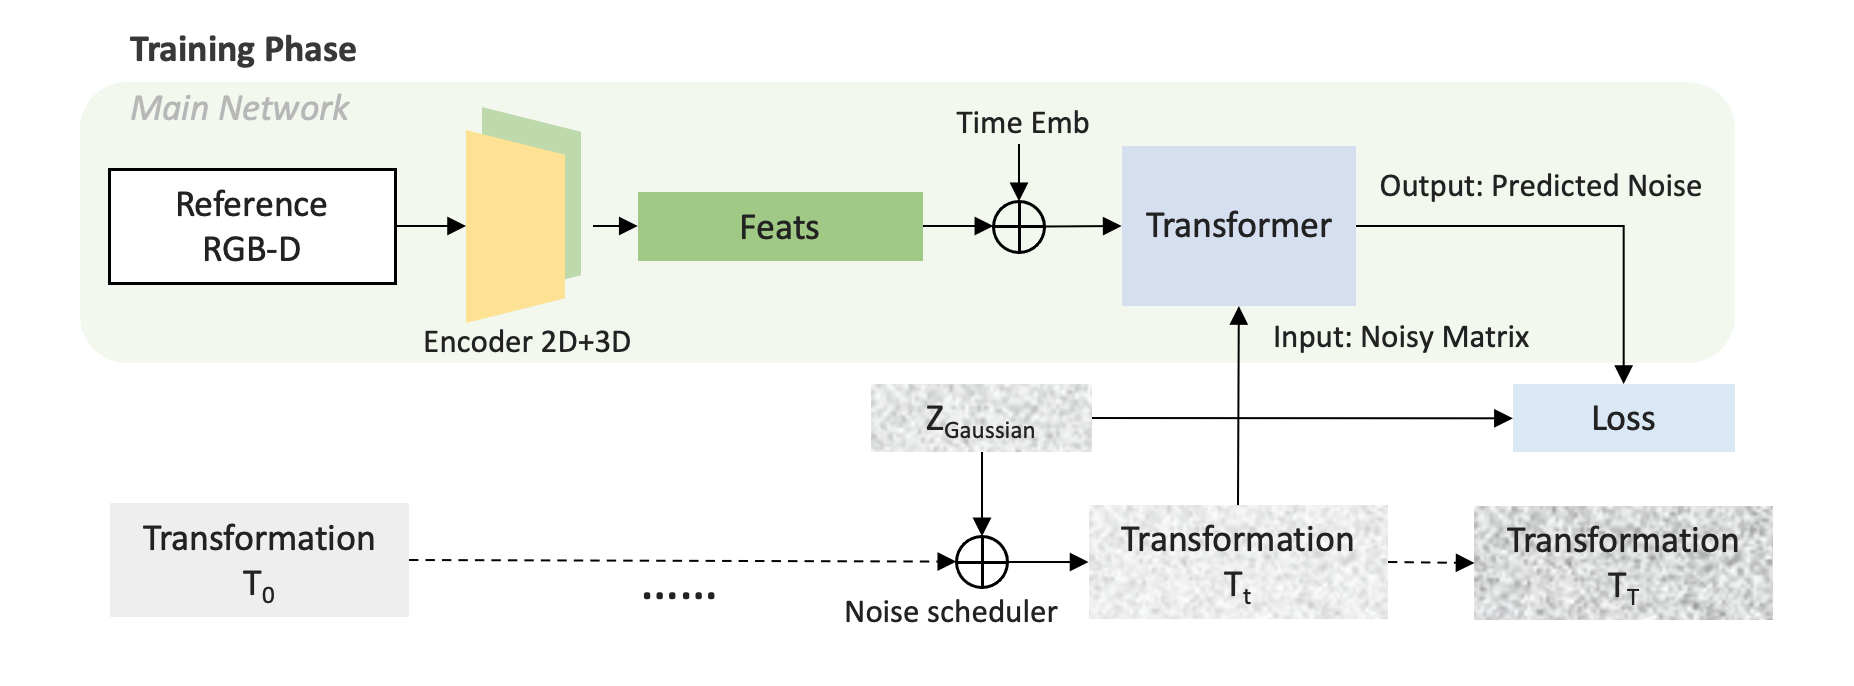
\includegraphics[scale=.23]{img/train.png}
	\caption{Structure of the training phase of the pose hypotheses diffusion}
	\label{img:train}
\end{figure}

\subsubsection{Sampling Phase}
Assuming that the denoiser is converged in the training phase, we can use the denoiser to iteratively generate the pose hypotheses with the randomly initialized the transformation $\mathbf{T}_{T}$. Same as the training phase, we need to provide the timestep $t$ and the guidance $\mathbf{y}$ to the backbone. Given a reference RGB-D image, we use the pretrained 2D and 3D encoder to extract the downstream features and concatinate them as the conditional embedding of the diffusion backbone. 

Since during the training phase, the network has learned the noise distribution conditioned each timestep embedding, so the denoiser has the capability to predict the noise $\boldsymbol{\epsilon}_{\theta}$ from $t=T$ to $t=0$. Then we can use the equation \ref{eq:reverse} to get the pose hypothesis $\mathbf{T}_{t-1}$ and repeat the process until we get the final pose hypothesis $\mathbf{T}_{0}$. 

In the training phase, we feed the network with batch of data that is different in the timestep $t$ and the guidance $\mathbf{y}$ (different reference images). During the sampling phase, we can easily make the batch size to one and only infer one pose hypothesis $\mathbf{T}_{0}$ for one reference input. Another efficient way is to simultaneously sample multiple pose hypotheses by batchifying the randomly initialized transformation and conditioned with the same reference input. And the mean of the sampled pose hypotheses can be more precisely estimated as the final pose estimation if the pose of the object is uniquely determined in the space. This can be switched that the batch of the random Gaussian initialization is conditioned with different reference inputs, which can infer multiple pose for different frames or different objects.

After the optional multi-hypotheses inference, we can further use some algorithms to refine the pose. In our model, we choose iterative closest point (ICP)\cite{121791} algorithm to refine the pose hypotheses and finally get the output transformation $\mathbf{T}_{r}$. The structure of the sampling process is shown in figure \ref{img:sample}. Details of each models in training phase and sampling phase will be introduced in next section.
\begin{figure}[h]
	\centering
	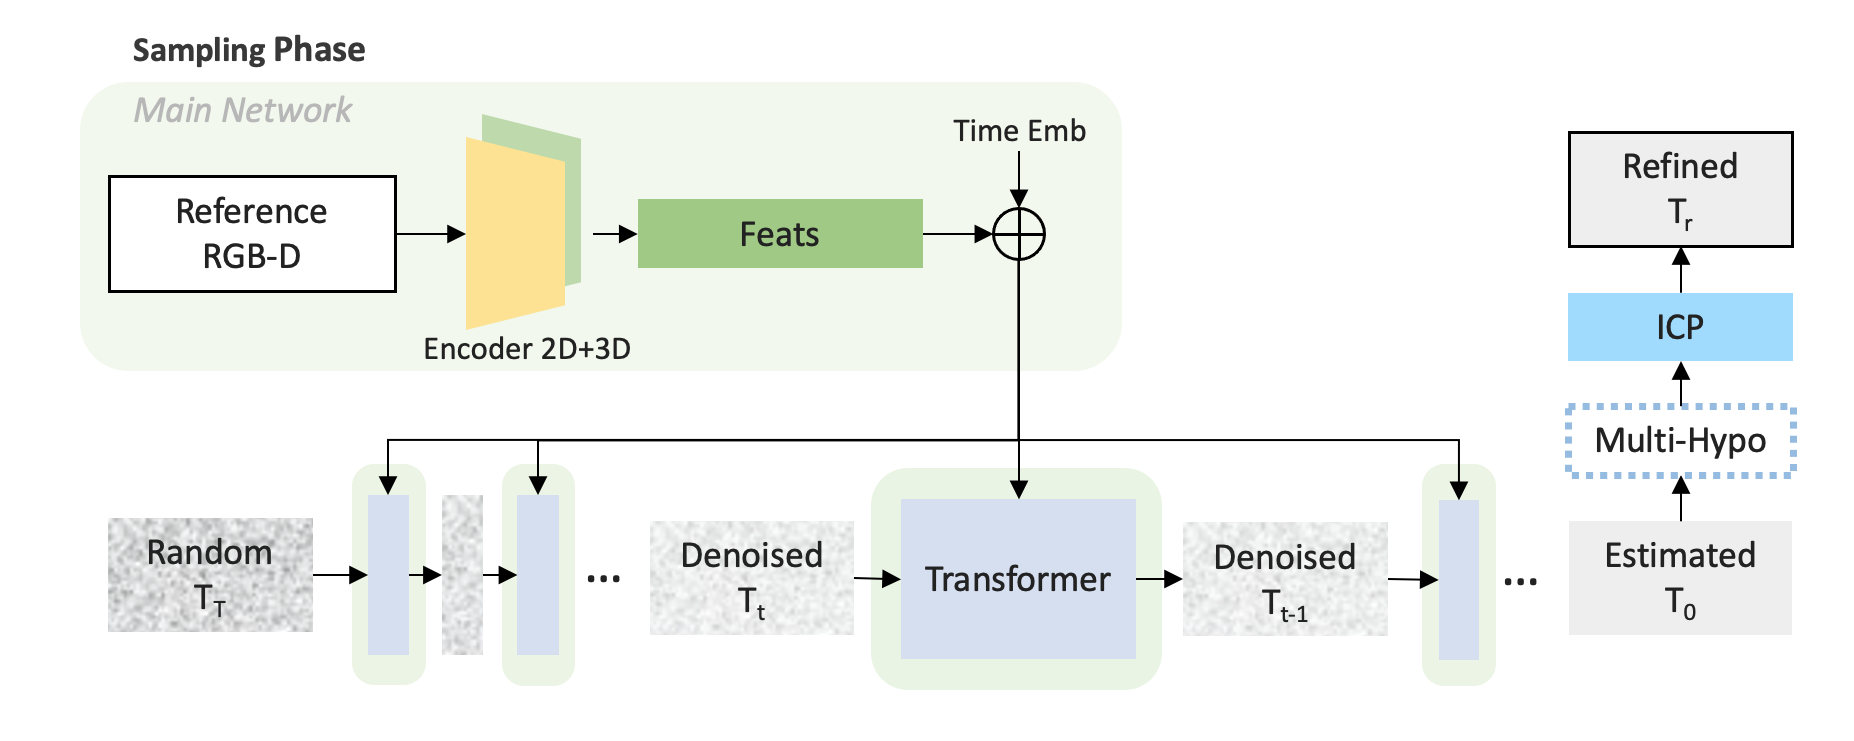
\includegraphics[scale=.23]{img/sample.png}
	\caption{Structure of the sampling phase of the pose hypotheses diffusion}
	\label{img:sample}
\end{figure}

\subsection{Models}
\subsubsection{Denoiser Network}
The following figure \ref{img:denoiser} illustrates the structure of our main network in diffusion model. As in previous section mentioned, the transformer encoder processes the translation and rotaion vector together with their position embedding conditioned with time embedding and 2D/3D feature embedding of the reference image and predicts the noise added at this timestep. 

It is worth mentioning that the fusion of 2D and 3D feature is not pointwise aligned, which means we don't extract the pointwise feature from the 2D and 3D domain and feed to the network. Instead of doing that, we seperately extract the global features and concatinate them together in order to reduce the difficulty of the convergence of the backbone with the tradeoff of the robustness and generalization of the model. This part of optimization will be discussed later.
\begin{figure}[h]
	\centering
	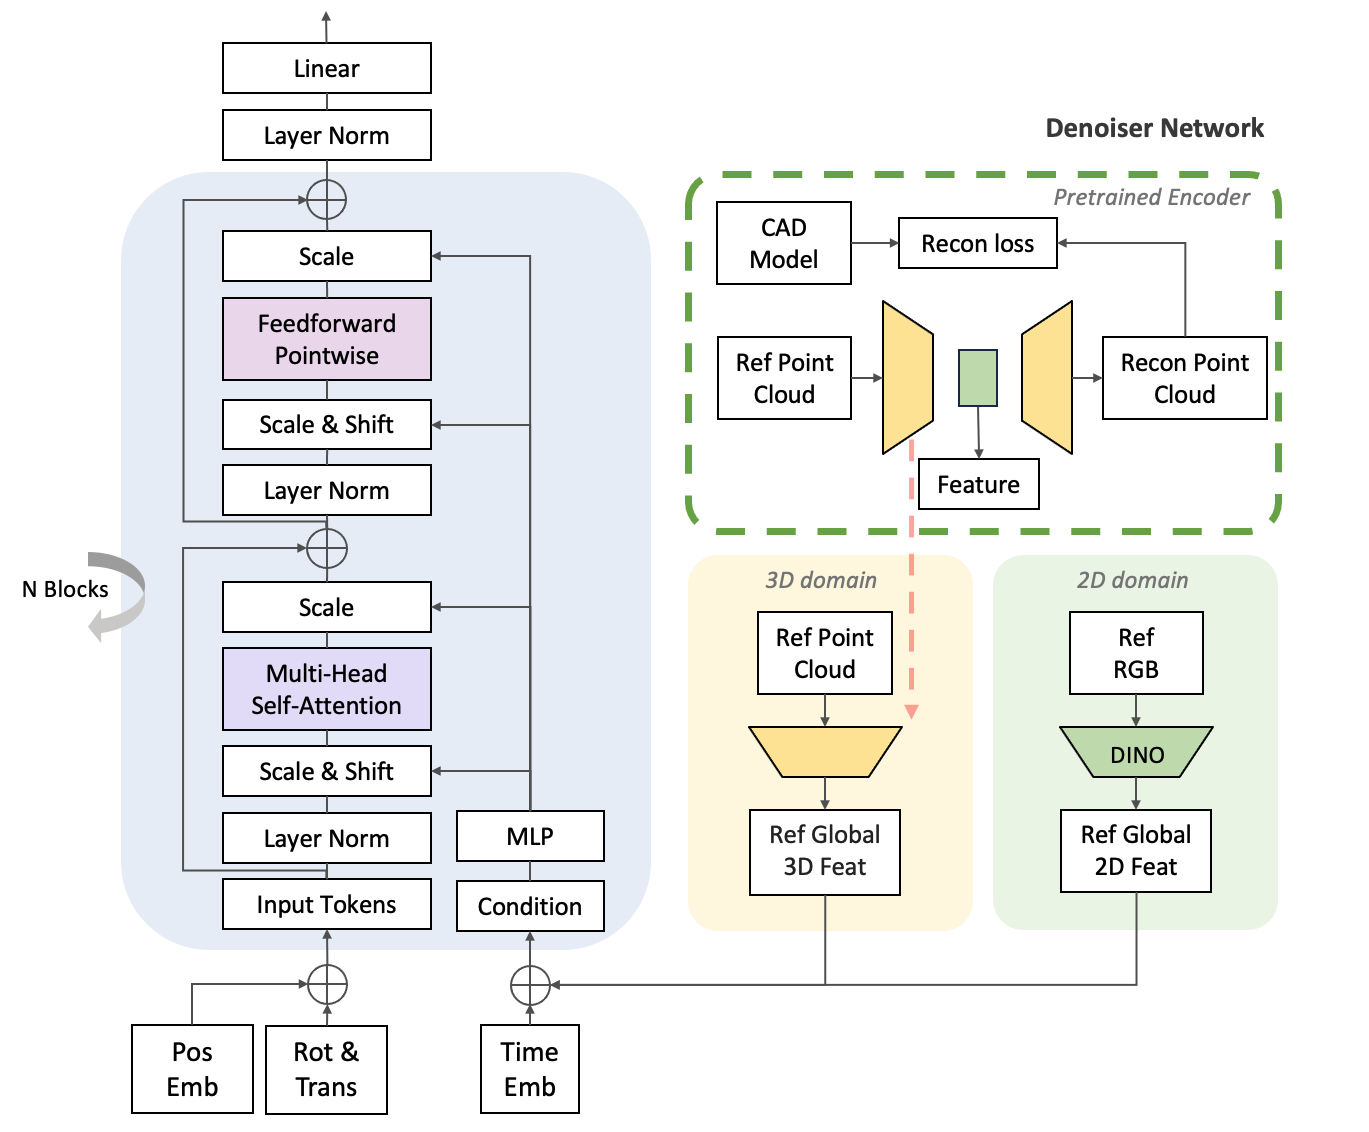
\includegraphics[scale=.30]{img/denoiser.png}
	\caption{Denoiser network with backbone and feature extractor}
	\label{img:denoiser}
\end{figure}

\subsubsection{Backbone}
A modified transformer encoder is utilized as the backbone of our diffusion model. The Transformer\cite{vaswani2023attention} is a sequence-to-sequence model that uses multi-head self-attension layers to understand the relevant token in the sequence and follows the encoder-decoder structure in the NLP tasks. However, in our case the encoder part is what we need to estimate the noise.

Similar to the vanilla transformer, our model consists of N stacked transformer encoder blocks. As shown in the left part of figure \ref{img:denoiser}, each block is made up of two sub-layers. The first is a multi-head self-attention mechanism, and the second is a simple, position-wise fully connected feed-forward network. We use residual connections around each of the two sub-layers and the Layer norm (LN) is applied before each sub-layer, which follows the design of Vision Transformer
 (ViT)\cite{dosovitskiy2021image}.
\begin{figure}[h]
	\centering
	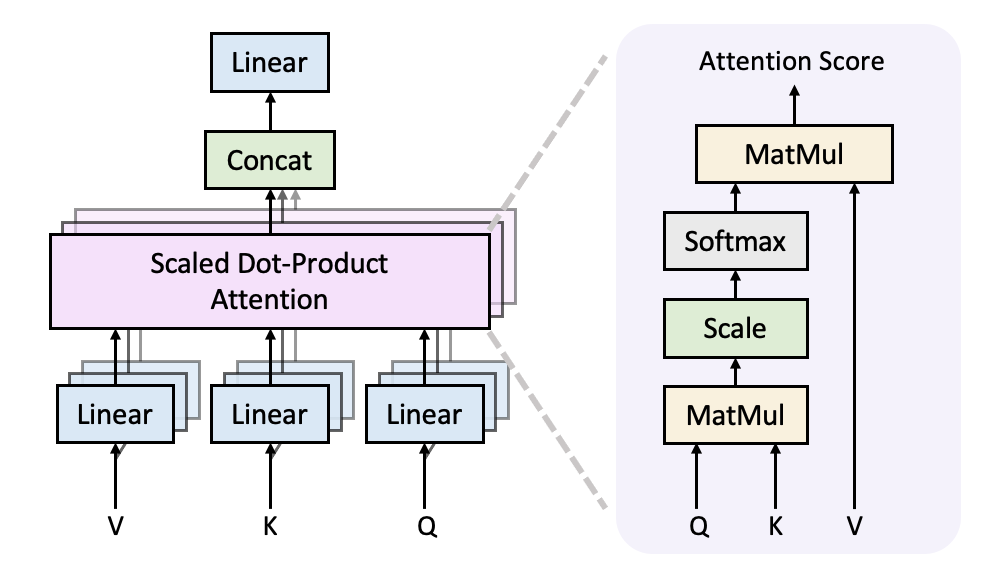
\includegraphics[scale=.30]{img/mhsa.png}
	\caption{Multi-head self-attention and scaled dot-product attention}
	\label{img:mhsa}
\end{figure}

The core of the transformer encoder is the multi-head self-attention mechanism, which is illustrated in figure \ref{img:mhsa}. First, we create three vectors from each input vector $\mathbf{x}_{i}$, namely the query vector $\mathbf{q}_{i}$, the key vector $\mathbf{k}_{i}$ and the value vector $\mathbf{v}_{i}$. These vectors are created by multiplying the input vector $\mathbf{x}_{i}$ with three matrices $\mathbf{W}^{Q}$, $\mathbf{W}^{K}$ and $\mathbf{W}^{V}$ respectively that we trained during the training phase. Then we use the scaled dot-product attention to calculate the output vector $\mathbf{y}_{i}$:
\begin{align}
  \mathbf{y}_{i} = \text{softmax}\left(\frac{\mathbf{q}_{i}\mathbf{k}_{i}^{T}}{\sqrt{d_{k}}}\right)\mathbf{v}_{i}
\end{align}
where $d_{k}$ is the dimension of the key vector $\mathbf{k}_{i}$. The scaled dot-product attention is the core of the transformer encoder and the multi-head self-attention is the extension of the scaled dot-product attention. The multi-head self-attention is defined as:
\begin{align}
  \text{MultiHead}(\mathbf{Q}, \mathbf{K}, \mathbf{V}) = \text{Concat}(\mathbf{h}_{1},...,\mathbf{h}_{n})\mathbf{W}^{O}
\end{align}
where $\mathbf{h}_{i} = \text{Attention}(\mathbf{Q}\mathbf{W}_{i}^{Q}, \mathbf{K}\mathbf{W}_{i}^{K}, \mathbf{V}\mathbf{W}_{i}^{V})$ and $\mathbf{W}_{i}^{Q}$, $\mathbf{W}_{i}^{K}$, $\mathbf{W}_{i}^{V}$ and $\mathbf{W}^{O}$ are the trainable parameters. The multi-head self-attention allows the model to jointly attend to information from different representation subspaces at different positions. With a linear projection at the end, the model is able to learn a more complex function.

To effectively process the conditional input, we use modified adaptive layer normalization (adaLN) to replace the original layer normalization in the transformer encoder which is introduced in \cite{perez2017film,Peebles2022DiT}. The learnable scale and shift parameters are regressed from the conditional input and applied in each sub-layer of the transformer encoder blocks. The modified transformer encoder block can be formulated as:
\begin{align}
  \mathbf{y}^{'} &= \alpha_{1}(\mathbf{c})\odot {\text{Attention}[\gamma_{1}(\mathbf{c})\odot N(\mathbf{x}) + \beta_{1}(\mathbf{c})]}\\
  \mathbf{y} &= \alpha_{2}(\mathbf{c})\odot {\text{FeedForward}[\gamma_{2}(\mathbf{c})\odot N(\mathbf{y}^{'}) + \beta_{2}(\mathbf{c})]}
\end{align}
where $\mathbf{y}$ is the output of the block, $\mathbf{y}^{'}$ is the intermediate expression after the first sub-layer,  $\mathbf{c}$ is the conditional input, $\alpha_{1}(\mathbf{c})$, $\alpha_{2}(\mathbf{c})$, $\beta_{1}(\mathbf{c})$, $\beta_{2}(\mathbf{c})$, $\gamma_{1}(\mathbf{c})$ and $\gamma_{1}(\mathbf{c})$ are the learnable parameters and $N$ is the layer normalization. The $\odot$ denotes the element-wise multiplication.

-----------------Reason for using transformer----------------

\subsubsection{Time Embedding and Postion Embedding}
Why we need time embedding and position embedding in our case? As the architecture of diffusion model determines that we need to let the network learn the influence of timestep on the noise estimation. So we have to encode the timestep information into the network. For the same reason, the sequence of the transformer input which is the transformation vector is also relevant and should be encoded, because the each bit of the vector represents the different meaning and can not be shuffled.

The way we embed time and position information is generally called positional encoding. It should satisfy the following conditions\cite{kazemnejad2019:pencoding}:
\begin{itemize}
  \item It should be unique and deterministic defined for each position (or timestep).
  \item The encoded distance between any two steps should be consistent across different timesteps.
  \item The value should be bounded and generalize to any input.
\end{itemize}
The most common positional encoding is the sine and cosine positional encoding\cite{vaswani2023attention}, which is defined as:
\begin{align}
  \text{PE}_{(pos, 2i)} &= \sin\left(\frac{pos}{10000^{2i/d_{model}}}\right)\\
  \text{PE}_{(pos, 2i+1)} &= \cos\left(\frac{pos}{10000^{2i/d_{model}}}\right)
\end{align}
where $pos$ is the position, $i$ is the dimension and $d_{model}$ is the dimension of the input vector. And we add a fully connected layer to the positional encoding to make it trainable. Figure \ref{img:pe} shows the 64-dimensional positional encoding for a sequence with length of 100 using the sine and cosine positional encoding.
\begin{figure}[h]
	\centering
	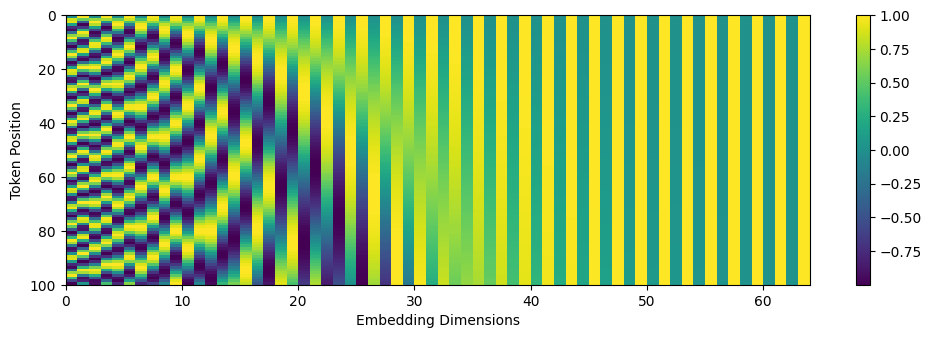
\includegraphics[scale=.65]{img/pe.png}
	\caption{The 64-dimensional positional encoding for a sequence with length of 100}
	\label{img:pe}
\end{figure}

\subsubsection{2D Feature Extractor}
As the 2D feature extractor, the self-supervised Vision Transformer
 with DINO\cite{caron2021emerging} is used. DINO is a self-supervised learning method that trains a Vision Transformer
 with a small set of negative examples. It is a contrastive learning method that maximizes the agreement between differently augmented views of the same image. The architecture of DINO shares the same overall structure with recent self-supervised approaches and also the similarites with knowledge distillation.

Knowledge distillation is a learning paradigm where a student network $g_{\theta_{s}}$ is trained to match the output of a given teacher network $g_{\theta_{t}}$, parameterized by $\theta_{s}$ and $\theta_{t}$ respectively. Given an input image $x$, both networks output probability distributions over $K$ dimensions denoted by $P_{s}$ and $P_{t}$. The probability $P$ is obtained by normalizing the output of the network $g$ with a softmax function. Given a fixed teacher network $g_{\theta_{t}}$, the student network $g_{\theta_{s}}$ is trained to minimize the cross-entropy loss between the two distributions w.r.t the student parameters $\theta_{s}$:
\begin{align}
  \mathop{min}_{\theta_{s}}H(P_{t}(x), P_{s}(x))
\end{align}
where $H(a,b)=-a \log b$ is the cross-entropy loss. And this optimizatiin problem is adapted to self-supervised learning by constructing different distorted views or crops of an image with multi-crop strategy. Making a set of two global views, $x_{1}^{g}$ and $x_{2}^{g}$ and several local views with smaller resolution, the loss function can be formulated as:
\begin{align}
  \mathop{min}_{\theta_{s}}\mathop{\sum}_{x\in \{x_{1}^{g},x_{2}^{g}\}} \ \mathop{\sum}_{x^{'}\in V \atop x^{'}\neq x}H(P_{t}(x), P_{s}(x^{'}))
\end{align}
The structure of the self-supervised architecture is shown in figure \ref{img:dino}. The model passes two different random transformations of the input image to both networks with same stucture but different parameters. The output of the teacher network is centered and a stop-gradient (sg) is applied on the teacher to let the gradients only propagate through the student network. The teacher parameters are updated with an exponential moving average (ema).
\begin{figure}
	\centering
	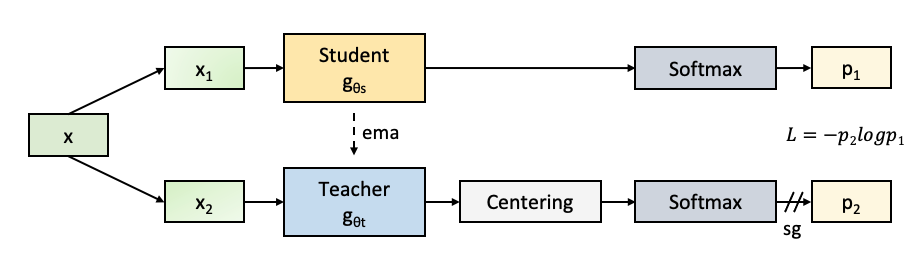
\includegraphics[scale=.38]{img/dino.png}
	\caption{Self-supervised architecture of DINO}
	\label{img:dino}
\end{figure}[h]

The backbone of the DINO is ViT\cite{dosovitskiy2021image}, which proved that the transformer architecture also performs well on the 2D vision tasks. The standard transformer processes 1D sequences, and in order to handle 2D images, the input is first flattened into a sequence of patches. For a input image $x\in R^{H\times W\times C}$ and patch size $p$, the patchified input can be denoted as $x_p\in R^{N\times(p^{2}C)}$ with the number of patches $N=\frac{HW}{p^{2}}$. The reason why the patches are feeded into the transformer rather the raw image is that it is relatively easier for the network to understand the relationship between the patches than the raw pixels.

Similar to the vanilla transformer for NLP tasks, the patches need to be embedded with the positional encoding. A standard learnable 1D postion embedding is used in the original paper. In order to solve the classification task with ViT, an extra token is add to the sequence of patches, which is called class token. An additional MLP layer is used for the classification. But for the downstream tasks like ours, we only need the latent feature from the transformer encoder output. The overview of the ViT model is shown in figure \ref{img:vit}, using the illustration in the original publication.
\begin{figure}[h]
	\centering
	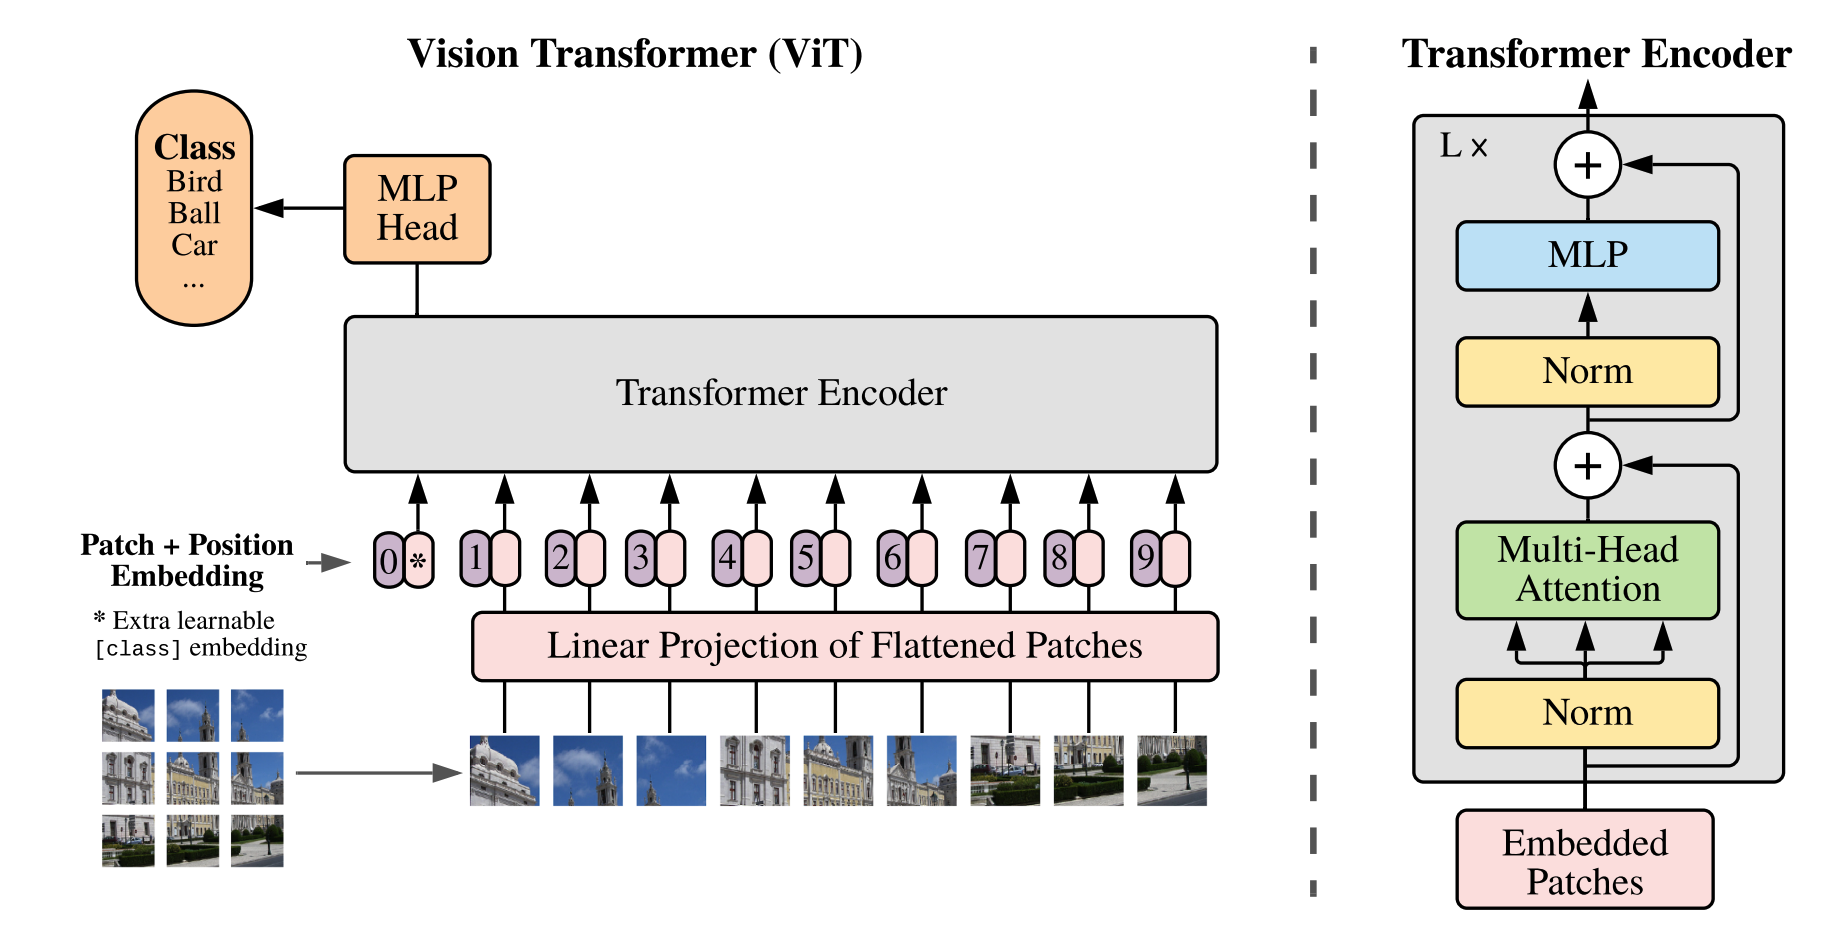
\includegraphics[scale=.23]{img/vit.png}
	\caption{Sturcture of the ViT model, image adapted from \cite{dosovitskiy2021image}}
	\label{img:vit}
\end{figure}

Compared with convolutional neural network which has a dominant position in the field of 2D vision tasks, the Vision Transformer has advantages as well as drawbacks under some scenarios. The transformer is more computationally expensive and requires more memory than the convolutional neural network. And the transformer is not as robust as the convolutional neural network in the case of small dataset. On the other hand, Vision Transformer architecture is more flexible and can be easily applied to different tasks with different input size. It offers a more natural way to process the 2D image, which is more similar to the human brain. And the transformer is more suitable for the tasks that require the global information of the image, such as the classification task. In our case, we use the Vision Transformer pretrained with DINO to extract the global feature of the reference image and feed it to the transformer encoder as the conditional embedding.

We directly use the weights of the model pretrained on ImageNet\cite{5206848}, because the 2D feature downstream network generalizes well on other datasets than 3D feature extractor, which has right now rare well generalized downstream backbone that can cover any 3D objects. Out of this reason, we train the 3D feature extractor from scratch on the dataset we use and this part will be introduced in next section.

\subsubsection{3D Feature Extractor}
Because of the permutation invariance of the point cloud, the 3D networks are differently constructed compared with the 2D networks. Famous works like PointNet\cite{qi2017pointnet} and PointNet++\cite{qi2017pointnet++} are the pioneer of the 3D deep learning. After that the convolutional neural network is also introduced to the 3D domain such as KPConv\cite{thomas2019kpconv}. 
\subsubsection{Multi-Hypotheses Inference}
\subsubsection{Pose Refinement}

\section{Experiments}
\subsection{Datasets}
\subsection{Training}
\subsection{Evaluation}
\chapter{Correspondance Diffusion}
\section{Introduction}
\section{Methodology}
\subsection{Pipeline}
\subsection{Models}
\section{Experiments}
\subsection{Datasets}
\subsection{Evaluation}
\chapter{Discussion}

\chapter{Conclusion}

\appendix
\chapter{Additionally}
You may do an appendix



% -------------------> end writing here <------------------------
% *****************************************************************
\listoffigures
\listoftables

\ifthenelse{\equal{\doclang}{german}}{
	\bibliographystyle{IEEEtran_ISSger}
}{
	\bibliographystyle{IEEEtran_ISS}
}
\bibliography{refs}

% *****************************************************************
%% Additional page with Declaration ("Eidesstattliche Erklrung");
%% completed automatically
\begin{titlepage}
      \vfill
      \LARGE \ifthenelse{\equal{\doclang}{german}}{\textbf{Erkl\"arung}}{\textbf{Declaration}}
      \vfill

      \ifthenelse{\equal{\doclang}{german}}{
         Hiermit erkl\"are ich, dass ich diese Arbeit selbstst\"andig verfasst und keine anderen als die angegebenen
         Quellen und Hilfsmittel benutzt habe.
      }
      {
         Herewith, I declare that I have developed and written the enclosed thesis entirely by myself and that I have not used sources or means except those declared.
      }

      \vspace{1cm}

      \ifthenelse{\equal{\doclang}{german}}{
         Die Arbeit wurde bisher keiner anderen Pr\"ufungsbeh\"orde vorgelegt und auch noch nicht ver\"offentlicht.
      }
      {
         This thesis has not been submitted to any other authority to achieve an academic grading and has not been published elsewhere.
      }

      \vfill

      
      Stuttgart, \signagedate
      \hfill
      \begin{tabular}{l}
          \hline
          \student
      \end{tabular}
\end{titlepage}



\end{document}
